% === Fig 1: Architecture (MANUAL, reused from paper_v2) ===
\begin{figure*}[t]
    \centering
    
\includegraphics[width=\textwidth]{figures/framework.png}
    \caption{Overview of the \textbf{InfoDelphi} framework.
    (a)~\textbf{Evidence Routing}: documents are ranked by BM25 relevance and
    distributed round-robin, constructing a shared public pool and disjoint private
    subsets for each agent.
    (b)~\textbf{Multi-Agent Deliberation}: agents exchange structured forecasts and
    rationales over two rounds, enabling private information to propagate.
    (c)~\textbf{Calibrated Aggregation}: final forecasts are pooled and passed through
    an asymmetric shrinkage transform toward a NO-leaning prior.}
    \label{fig:arch}
\end{figure*}

% === Fig 2: Herding dynamics ===
\begin{figure}[t]
    \centering
    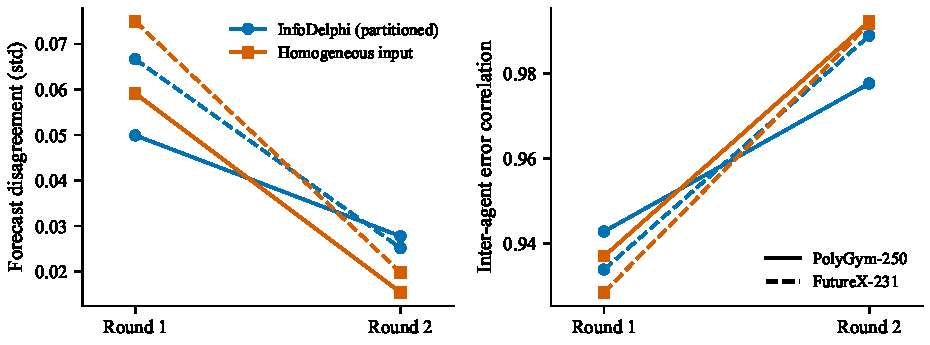
\includegraphics[width=\columnwidth]{figures/fig2_herding.pdf}
    \caption{Deliberation dynamics with and without information asymmetry.
    Left: mean per-question standard deviation of agent forecasts; right: mean
    pairwise inter-agent error correlation. Under homogeneous input, deliberation
    collapses forecast diversity (herding); partitioned evidence preserves
    independent signal after deliberation on both datasets.}
    \label{fig:herding}
\end{figure}

% === Fig 3: Calibration study ===
\begin{figure}[t]
    \centering
    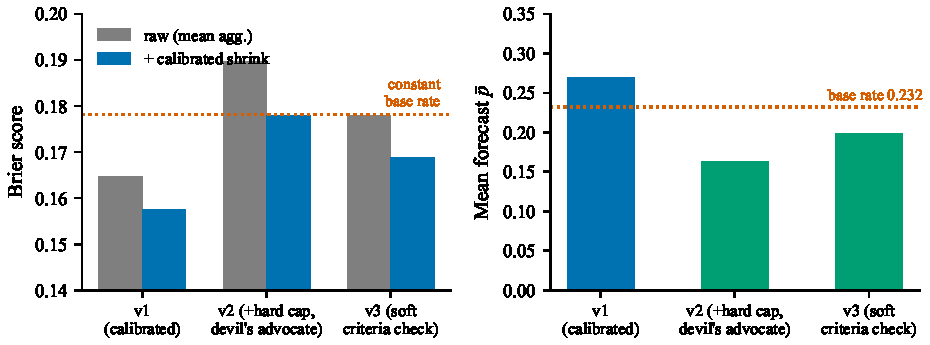
\includegraphics[width=\columnwidth]{figures/fig3_calibration.pdf}
    \caption{Prompt-level vs.\ aggregation-level calibration on
    \textsc{PolyGym}-250. Left: Brier score of three calibration prompts, with and
    without aggregation-level shrinkage. Right: mean forecast $\bar p$ against the
    empirical base rate. Skeptical prompt wording (v2, v3) depresses the entire
    forecast distribution below the base rate and hurts accuracy in the mid-band,
    whereas asymmetric shrinkage corrects overconfidence where it occurs.}
    \label{fig:calibration}
\end{figure}

% === Tables: \input from figures/ ===
% Tab 1: \begin{table*}[t]
\centering
\small
\caption{Main results on \textsc{PolyGym}-250 and FutureX-231. All methods use \texttt{gpt-5.4-mini} over the same fixed pre-resolution evidence pools. AUC is invariant to monotone recalibration, so it isolates ranking skill from the calibration layer (identical for our raw and full rows). $\dagger$: InfoDelphi (full) is significantly better under a paired bootstrap over questions (5{,}000 resamples; 95\% CI of the Brier difference excludes 0; Appendix Table~\ref{tab:significance}). Best in \textbf{bold}.}
\label{tab:main}
\begin{tabular}{lcccccc}
\toprule
 & \multicolumn{3}{c}{\textsc{PolyGym}-250} & \multicolumn{3}{c}{FutureX-231} \\
\cmidrule(lr){2-4}\cmidrule(lr){5-7}
Method & Brier$\,\downarrow$ & Acc$\,\uparrow$ & AUC$\,\uparrow$ & Brier$\,\downarrow$ & Acc$\,\uparrow$ & AUC$\,\uparrow$ \\
\midrule
\multicolumn{7}{l}{\textit{Single-agent}} \\
Chain-of-Thought~\citep{wei2022chain}$^\dagger$ & 0.2063 & 0.696 & 0.678 & 0.2611 & 0.606 & 0.663 \\
Self-Consistency~\citep{wangself}$^\dagger$ & 0.1965 & 0.712 & 0.699 & 0.2713 & 0.550 & 0.630 \\
Sequential Bayesian~\citep{shi2023language}$^\dagger$ & 0.2523 & 0.540 & 0.591 & 0.3043 & 0.485 & 0.534 \\
Superforecaster~\citep{karger2024forecastbench}$^\dagger$ & 0.1937 & 0.700 & 0.722 & 0.2596 & 0.636 & 0.672 \\
Halawi et al.~\citep{halawi2024approaching}$^\dagger$ & 0.1944 & 0.716 & 0.711 & 0.2654 & 0.567 & 0.629 \\
\midrule
\multicolumn{7}{l}{\textit{Multi-agent, homogeneous input}} \\
Standard Debate~\citep{du2023improving}$^\dagger$ & 0.1815 & 0.720 & 0.711 & 0.2433 & 0.602 & 0.694 \\
MoA~\citep{wangmixture}$^\dagger$ & 0.1905 & 0.720 & 0.716 & 0.2944 & 0.545 & 0.599 \\
Crowd Ensemble~\citep{schoenegger2024wisdom}$^\dagger$ & 0.1992 & 0.700 & 0.700 & 0.2888 & 0.524 & 0.599 \\
AIA Forecaster~\citep{alur2025aia}$^\dagger$ & 0.1897 & 0.704 & 0.729 & 0.2764 & 0.550 & 0.635 \\
\midrule
\multicolumn{7}{l}{\textit{Ours}} \\
InfoDelphi w/o calibrated shrink & 0.1647 & \textbf{0.748} & \textbf{0.757} & 0.2212 & 0.688 & \textbf{0.711} \\
\textbf{InfoDelphi (full)} & \textbf{0.1575} & 0.744 & \textbf{0.757} & \textbf{0.2006} & \textbf{0.701} & \textbf{0.711} \\
\bottomrule
\end{tabular}
\end{table*}
   (label tab:main)
% Tab 2: \begin{table}[t]
\centering
\small
\caption{Component ablation (Brier$\,\downarrow$). Each row removes one component from the full system. ``$-$ asymmetry'' gives every agent the full evidence pool ($\rho{=}1$, full sharing) with the same calibrated prompt, i.e., the Standard Debate configuration of our pipeline. Paired 95\% CIs for each removal are given in the text.}
\label{tab:ablation}
\begin{tabular}{lcc}
\toprule
Configuration & \textsc{PolyGym} & FutureX \\
\midrule
InfoDelphi (full) & \textbf{0.1575} & \textbf{0.2006} \\
$-$ calibrated shrink (mean agg.) & 0.1647 & 0.2212 \\
$-$ deliberation (round 1 only) & 0.1698 & --- \\
$-$ information asymmetry & 0.1815 & 0.2433 \\
\bottomrule
\end{tabular}
\end{table}
       (label tab:ablation)
% Tab 3: \begin{table}[t]
\centering
\small
\caption{Targeted retrieval augmentation on the 106 Sports questions of \textsc{PolyGym}-250 (InfoDelphi full; paired bootstrap vs.\ original evidence, 5{,}000 resamples). Neither augmentation yields a significant improvement.}
\label{tab:sports}
\begin{tabular}{lccc}
\toprule
Evidence & Brier$\,\downarrow$ & AUC$\,\uparrow$ & $\Delta$Brier [95\% CI] \\
\midrule
Original & 0.1908 & 0.696 & --- \\
$+$ opponent identity & 0.1890 & 0.690 & -0.0018 [-0.010, +0.006] \\
$+$ opponent odds/form & 0.1873 & 0.720 & -0.0035 [-0.013, +0.005] \\
\bottomrule
\end{tabular}
\end{table}
         (label tab:sports)
% Tab 4 (App): \begin{table*}[t]
\centering
\small
\caption{Control experiment: applying our calibrated-shrink transform ($p_0{=}0.30$, $w_{\mathrm{lo}}{=}0.8$, $w_{\mathrm{hi}}{=}0.5$) to every baseline's output. Shrinkage improves all methods; the ranking is preserved and InfoDelphi remains best on both datasets, although several pairwise gaps are no longer individually significant (n.s.). $\Delta$ is the paired Brier difference of InfoDelphi (full) vs.\ the shrunk baseline (negative favors ours).}
\label{tab:shrink_control}
\begin{tabular}{lcccccc}
\toprule
 & \multicolumn{3}{c}{\textsc{PolyGym}-250} & \multicolumn{3}{c}{FutureX-231} \\
\cmidrule(lr){2-4}\cmidrule(lr){5-7}
Method & raw & $+$shrink & $\Delta$ [95\% CI] & raw & $+$shrink & $\Delta$ [95\% CI] \\
\midrule
Chain-of-Thought & 0.2063 & 0.1738 & $-0.016$ $[-0.029, -0.003]$ & 0.2611 & 0.2158 & $-0.015$ $[-0.033, +0.003]$\,n.s. \\
Self-Consistency & 0.1965 & 0.1706 & $-0.013$ $[-0.025, -0.002]$ & 0.2713 & 0.2218 & $-0.021$ $[-0.038, -0.004]$ \\
Sequential Bayesian & 0.2523 & 0.2025 & $-0.045$ $[-0.059, -0.030]$ & 0.3043 & 0.2411 & $-0.041$ $[-0.060, -0.021]$ \\
Superforecaster & 0.1937 & 0.1665 & $-0.009$ $[-0.021, +0.004]$\,n.s. & 0.2596 & 0.2146 & $-0.014$ $[-0.031, +0.003]$\,n.s. \\
Halawi et al. & 0.1944 & 0.1693 & $-0.012$ $[-0.024, +0.000]$\,n.s. & 0.2654 & 0.2224 & $-0.022$ $[-0.039, -0.004]$ \\
Standard Debate & 0.1815 & 0.1650 & $-0.008$ $[-0.015, +0.000]$\,n.s. & 0.2433 & 0.2064 & $-0.006$ $[-0.022, +0.011]$\,n.s. \\
MoA & 0.1905 & 0.1670 & $-0.010$ $[-0.021, +0.002]$\,n.s. & 0.2944 & 0.2326 & $-0.032$ $[-0.049, -0.015]$ \\
Crowd Ensemble & 0.1992 & 0.1701 & $-0.013$ $[-0.025, -0.000]$ & 0.2888 & 0.2309 & $-0.030$ $[-0.048, -0.012]$ \\
AIA Forecaster & 0.1897 & 0.1651 & $-0.008$ $[-0.019, +0.004]$\,n.s. & 0.2764 & 0.2223 & $-0.022$ $[-0.039, -0.003]$ \\
\midrule
InfoDelphi (full) & 0.1647 & \textbf{0.1575} & --- & 0.2212 & \textbf{0.2006} & --- \\
\bottomrule
\end{tabular}
\end{table*}
 (label tab:shrink_control)
% Tab 5 (App): \begin{table*}[t]
\centering
\small
\caption{Paired bootstrap comparison of InfoDelphi (full) against each baseline (5{,}000 resamples over questions, seed 0). $\Delta$Brier $<0$ favors InfoDelphi; all 95\% CIs exclude zero.}
\label{tab:significance}
\begin{tabular}{lcc}
\toprule
Baseline & \textsc{PolyGym}-250 $\Delta$Brier [95\% CI] & FutureX-231 $\Delta$Brier [95\% CI] \\
\midrule
Chain-of-Thought & $-0.0488$ $[-0.0756, -0.0217]$ & $-0.0606$ $[-0.0958, -0.0258]$ \\
Self-Consistency & $-0.0390$ $[-0.0619, -0.0149]$ & $-0.0707$ $[-0.1032, -0.0381]$ \\
Sequential Bayesian & $-0.0948$ $[-0.1209, -0.0681]$ & $-0.1037$ $[-0.1402, -0.0684]$ \\
Superforecaster & $-0.0362$ $[-0.0620, -0.0097]$ & $-0.0591$ $[-0.0941, -0.0248]$ \\
Halawi et al. & $-0.0370$ $[-0.0615, -0.0123]$ & $-0.0648$ $[-0.0966, -0.0338]$ \\
Standard Debate & $-0.0240$ $[-0.0416, -0.0064]$ & $-0.0427$ $[-0.0761, -0.0114]$ \\
MoA & $-0.0331$ $[-0.0573, -0.0086]$ & $-0.0938$ $[-0.1295, -0.0580]$ \\
Crowd Ensemble & $-0.0418$ $[-0.0662, -0.0167]$ & $-0.0882$ $[-0.1224, -0.0534]$ \\
AIA Forecaster & $-0.0323$ $[-0.0566, -0.0077]$ & $-0.0758$ $[-0.1103, -0.0409]$ \\
\bottomrule
\end{tabular}
\end{table*}
   (label tab:significance)
